\subsection{Summary of findings}

\begin{frame}{Research objectives}
    Based on the challenges mentioned above, we define the main purposes of this study are as follow: 
    \begin{enumerate}[A]
        \item {\color{blue}to identify the effectiveness of the RKB approach for collaborative concept mapping in a practical classroom};
        \begin{enumerate}
            \item Collaborative product evaluation
            \item  Exploring students' perceptions toward the activity
        \end{enumerate}
        
        \item {\color{blue} to investigate how individual differences in prior knowledge has potentially influence collaborative-learning effectiveness and the students' perceptions toward the activities}; 
        \begin{enumerate}[3]
            \item Analyzing the effect of different group formation on collaboration
        \end{enumerate}
        
        \item {\color{blue} to analyze how similarity of individual knowledge and comprehension  of partner's representation could predict the final collaborative products}.
        \begin{enumerate}[4]
            \item Predicting group outcomes based on individual maps
        \end{enumerate}
    \end{enumerate} 
\end{frame}

\begin{frame}{Key findings from all conducted studies}
    \begin{enumerate}
    \item <1-> [RO:A] The students build \textcolor{teal}{high-quality group products}. 
    \item <2-> [RO:A] The students perceive \textcolor{teal}{positive responses} toward the activities. 
    \item <3-> [RO:B] Group formation based on the similarity of individual 
    knowledge \textcolor{teal}{does not significantly affect the individual-to-group 
    transfer of knowledge and the group outcomes}, however, 
    the students may provide \textcolor{purple}{less positive responses} toward the activities.
    \item <4-> [RO:C] \textcolor{teal}{The comprehension of partner's representation is a 
    stronger predictor} to estimate the group outcomes compare to the similarity of initial knowledge. 
\end{enumerate}  
\end{frame}

\subsection{Study limitations and directions for future works}
\begin{frame}{Limitations of the current study}
    \begin{itemize}
        \item <1>\textcolor{purple}{Generalizability of findings}\\
        {\small sample: 44 participants, subject: Math., 2 hours experimental session}
        \item <2>\textcolor{purple}{Single group study designs}\\
        {\small there is no control group}
    \end{itemize}
\end{frame}

\begin{frame}{Limitations of the current study (cont'd)}
    \begin{itemize}
        \item \textcolor{purple}{The evaluation of learning effectiveness at a group and interaction level}\\
        {\small an assessment of learning effect at the individual level is 
        necessary to comprehend the current findings}
    \end{itemize}
\end{frame}

\begin{frame}{Another potential future works}
    \begin{itemize}
        \item Development of a supporting function for collaboration based on the reconstructed maps\\
        \item Bigger group size (more than 2 people)\\
    \end{itemize}
\end{frame}

\begin{frame}{Summary of this study}
   \begin{figure}[tb]
       \begin{center}
           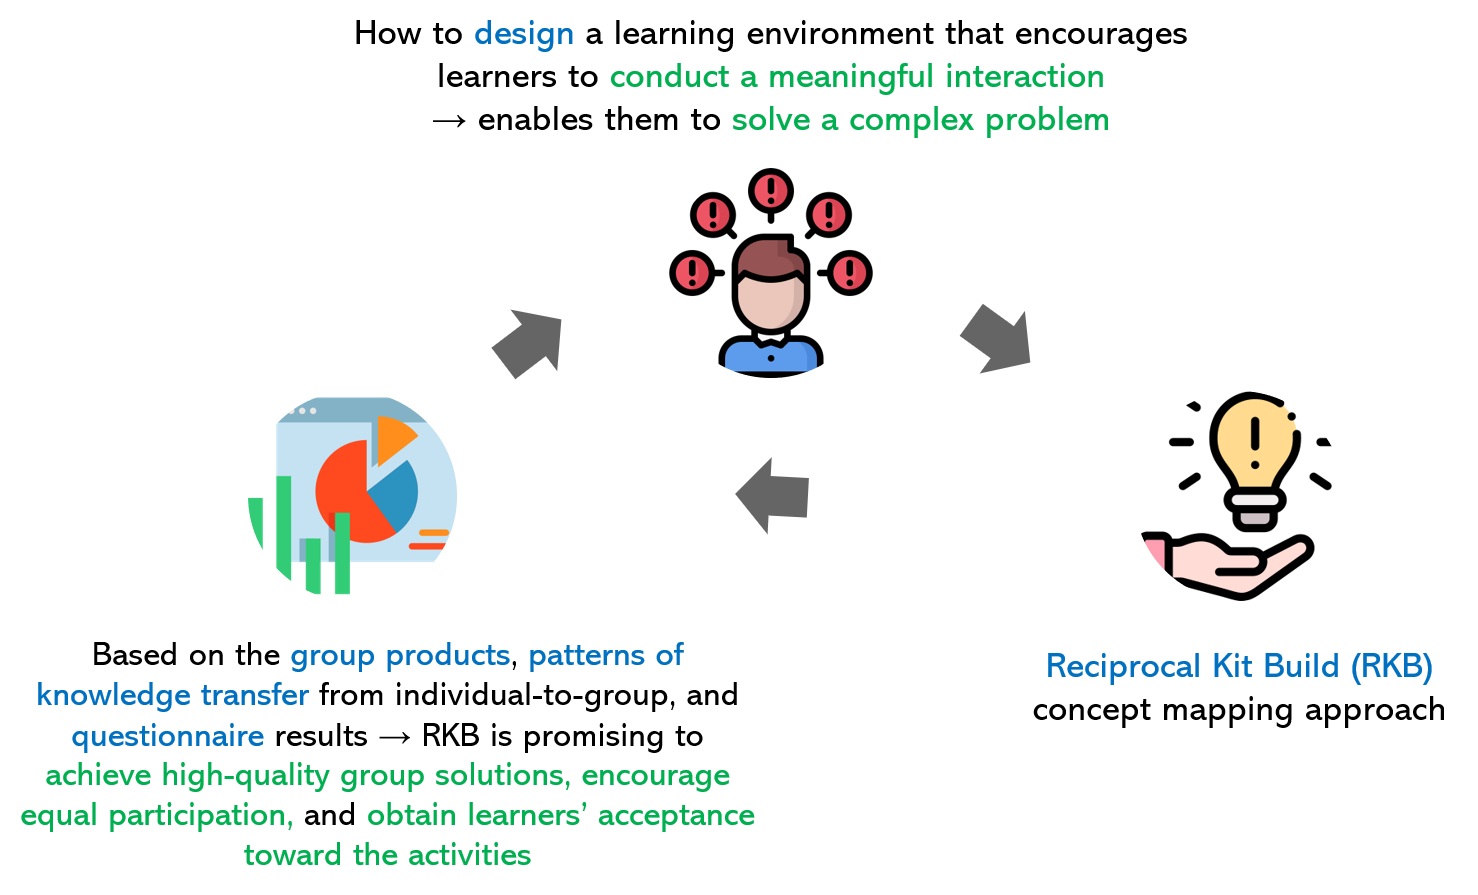
\includegraphics[width=110mm]{images/summary.png} 
       \end{center}
   \end{figure}
\end{frame}


\begin{frame}{Publication: Journal articles}
%\resizebox{\textwidth}{!}{%
\begin{tabular}{p{15mm}p{80mm}}
    \tiny{\color{blue}{RPTEL 2020}} & {\small \underline{Sadita,  L.},  Hirashima,  T.,  Hayashi,  Y.,  Furtado,  P.  G.,  Junus,  K.,  and Santoso,  H.  B.  (2020).   The  Effect  of  Differences  in  Group  Composition on Knowledge Transfer, Group Achievement and Learners' Affective Responses During Reciprocal Concept Mapping With The Kit-Build Approach. \textit{Research and Practice in Technology Enhanced Learning}, 15(13).  \href{https://doi.org/10.1186/s41039-020-00133-9}{10.1186/s41039-020-00133-9.}}\\
    \tiny{\color{blue}{IEICE 2020}} & {\small\underline{Sadita, L.}, Furtado, P. G. F., Hirashima, T., and Hayashi, Y. (in press). Analysis of The Similarity of Individual Knowledge and The Comprehension of Partner’s Representation during Collaborative Concept Mapping with Reciprocal Kit Build Approach. \textit{IEICE  TRANSACTIONS  on Information and Systems}, E103-D(7)}. 
\end{tabular}
%}
\end{frame}

\begin{frame}[allowframebreaks]{Publication: International conference papers}
\begin{tabular}{p{15mm}p{80mm}}
    \tiny{\color{blue}{ICCE 2018}} & {\small\underline{Sadita, L.}, Hirashima, T., Hayashi, Y., Wunnasri, W., Pailai, J., Junus, K.,and Santoso, H. B. (2018). Preliminary Study on the Use of Reciprocal Kit Build for Collaborative Learning.  In \textit{The  26th  International  Conference on Computers in Education (ICCE 2018)}, pages 133–142.}\\
    
    \tiny{\color{blue}{ICCE 2019}} & {\small \underline{Sadita,  L.},  Hirashima,  T.,  Hayashi,  Y.,  Furtado,  P.  G.,  Junus,  K.,  and Santoso, H. B. (2019c).  Reciprocal Kit Build Approach for Peer-to-peer Communication:  Relationship between Similarities on Knowledge, Transfer  of  Knowledge,  and  Affective  Responses. In \textit{The  27th International Conference  on  Computers  in  Education  (ICCE  2019)},  volume  1,  pages 101–110.}\\
\end{tabular}

\begin{tabular}{p{15mm}p{80mm}}
    \tiny{\color{blue}{ICCE-DSC 2019}} & {\small \underline{Sadita, L.}, Hirashima, T., and Hayashi, Y. (2019).  Reciprocal Kit Build Concept Map:  An Activity Designed to Encourage Learning at Boundary in Collaborative Situation.  In \textit{The 27th International Conference on Computers in Education (ICCE 2019)}, volume 2, pages 779–782.}
\end{tabular}
\end{frame}

\begin{frame}{Publication: Local conference papers}
\begin{tabular}{p{15mm}p{80mm}}
    \tiny{\color{blue}{ALST 2019}} &\underline{Sadita, L.}, Hirashima, T., Hayashi, Y., et al. (2019b). Reciprocal Kit Build:Boundary Crossing with Concept Map for Collaborative Knowledge Construction. 先進的学習科学と工学研究会, 86:50–55.
\end{tabular}
\end{frame}



\begin{frame}{}
    Thank you for your attention :-)
\end{frame}

